 \documentclass[xcolor=dvipsnames,table]{beamer}

\usepackage{latexsym}
\usepackage[utf8]{inputenc}
\usepackage[brazil]{babel}
\usepackage{amssymb}
\usepackage{amsmath}
\usepackage{stmaryrd}
\usepackage{fancybox}
\usepackage{datetime}
\usepackage[T1]{fontenc}
\usepackage{graphicx}
\usepackage{graphics}
\usepackage{url}
\usepackage{algorithmic}
\usepackage{algorithm}
\usepackage{acronym}
\usepackage{array}
\usepackage{tikz}

\usepackage{enumitem}

\newtheorem{definicao}{Definio}
\newcommand{\tab}{\hspace*{2em}}

\mode<presentation>
{
  \definecolor{colortexto}{RGB}{0,0,0}
 
  \setbeamertemplate{background canvas}[vertical shading][ bottom=white!10,top=white!10]
  \setbeamercolor{normal text}{fg=colortexto} 

  \usetheme{Warsaw}
}

\title{Agentes de Busca Informada}  

\author{
  Esdras Lins Bispo Jr. \\ \url{bispojr@ufj.edu.br}
  } 
 \institute{
  Inteligência Artificial \\Bacharelado em Ciência da Computação}
\date{\textbf{09 de setembro de 2026} }

\logo{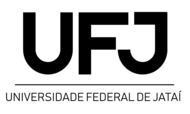
\includegraphics[width=1.5cm]{images/ufjJataiLogo.png}}

\begin{document}

	\begin{frame}
		\titlepage
	\end{frame}

	\AtBeginSection{
		\begin{frame}{Sumário}%[allowframebreaks]{Sumário}
    		\tableofcontents[currentsection]
    		%\tableofcontents[currentsection, hideothersubsections]
		\end{frame}
	}

	\begin{frame}{Plano de Aula}
		\tableofcontents
		%\tableofcontents[hideallsubsections]
	\end{frame}
	
	\section{Instrução pelos Colegas}
	

    \begin{frame}{Pesquisa 003}
		\begin{block}{[P011]}
			Como foi o estudo prévio?
		\end{block}
		\begin{enumerate}[label=(\Alph*)]
			\item Bom
			\item Razoável
			\item Difícil de entender
			\item Não consegui estudar
		\end{enumerate}
	\end{frame}

    \subsection{Busca Informada}

\begin{frame}{Da busca cega à busca informada}

    \begin{block}{Busca cega}

        A busca não utiliza informações específicas sobre o domínio

        para decidir qual nó parece mais promissor.

    \end{block}

    \begin{block}{Busca informada}

        A busca utiliza \textbf{conhecimento sobre o problema} para

        orientar a escolha do próximo nó a ser expandido.

    \end{block}

    \begin{center}

        \Large

        \textbf{fronteira}

        $\;\longrightarrow\;$

        \textbf{avaliação dos nós}

        $\;\longrightarrow\;$

        \textbf{próximo nó}

    \end{center}

\end{frame}

\begin{frame}{Busca pela melhor escolha}

    \begin{block}{Ideia central}

        Atribuir a cada nó da fronteira um valor de avaliação

        e expandir aquele considerado mais promissor.

    \end{block}

    \begin{center}

        \Large

        \[
        \boxed{\text{expandir o nó com melhor avaliação}}
        \]

    \end{center}

    \begin{block}{O ponto importante}

        A estratégia de busca depende de \textbf{como a avaliação é definida}.

        Diferentes funções de avaliação podem produzir diferentes

        comportamentos de busca.

    \end{block}

\end{frame}

\begin{frame}{Questão 009}

    \small

    \begin{block}{[Q009]}

        Duas buscas começam com o mesmo estado inicial e possuem

        exatamente a mesma fronteira de nós. Entretanto, elas escolhem

        nós diferentes para a próxima expansão.

        Qual situação explica melhor essa diferença?

    \end{block}

    \begin{enumerate}[label=(\Alph*)]

        \item Uma delas necessariamente encontrou uma representação

        diferente para o mesmo problema.

        \item Uma delas pode estar utilizando uma função de avaliação

        diferente para ordenar os nós da fronteira.

        \item Uma delas possui necessariamente mais estados disponíveis

        para explorar.

        \item Uma delas deve ter chegado a uma solução antes da outra.

    \end{enumerate}

\end{frame}

\subsection{Busca Gulosa e Busca A*}

\begin{frame}{Busca Gulosa: olhar para o objetivo}

    \begin{block}{Heurística}

        A função $h(n)$ estima o custo para chegar do nó $n$

        até o objetivo.

    \end{block}

    \begin{center}

        \Large

        \[
        \boxed{f(n)=h(n)}
        \]

    \end{center}

    \begin{block}{Busca gulosa}

        A fronteira é ordenada apenas pela estimativa do

        \textbf{custo restante}.

        \medskip

        \centering

        ``Qual nó parece estar mais próximo do objetivo?''

    \end{block}

\end{frame}

\begin{frame}{Busca A*: passado + futuro}

    \begin{block}{Duas informações}

        $g(n)$: custo real para chegar ao nó $n$.

        \[
        h(n): \text{estimativa do custo restante}
        \]

    \end{block}

    \begin{center}

        \Large

        \[
        \boxed{f(n)=g(n)+h(n)}
        \]

    \end{center}

    \begin{block}{Ideia central}

        A A* não considera apenas onde o nó parece estar em relação

        ao objetivo, mas também \textbf{quanto já foi gasto para chegar até ele}.

    \end{block}

\end{frame}

\begin{frame}{Questão 010}

    \begin{block}{[Q010]}

        Uma busca precisa escolher entre dois nós da fronteira.

        Para o nó $A$, temos $g(A)=20$ e $h(A)=10$.

        Para o nó $B$, temos $g(B)=5$ e $h(B)=20$.

        Um algoritmo utiliza $g(n)+h(n)$ para decidir qual nó expandir.

        Qual nó será escolhido?

    \end{block}

    \begin{enumerate}[label=(\Alph*)]

        \item $A$, porque sua estimativa de custo restante é menor.

        \item $A$, porque foi necessário percorrer mais caminho até alcançá-lo.

        \item $B$, porque sua avaliação total é menor.

        \item $B$, porque sua distância estimada até o objetivo é maior.

    \end{enumerate}

\end{frame}

\begin{frame}{Questão 011}

    \small

    \begin{block}{[Q011]}

        Uma busca gulosa chega a um estado que parece muito próximo

        do objetivo. Porém, para chegar até esse estado, ela percorreu

        um caminho bastante caro.

        O que explica por que a A* pode escolher outro caminho?

    \end{block}

    \begin{enumerate}[label=(\Alph*)]

        \item A A* ignora a distância estimada até o objetivo e considera

        apenas o caminho que já foi percorrido.

        \item A A* considera tanto o custo acumulado quanto uma

        estimativa do custo que ainda falta.

        \item A A* sempre escolhe o nó que está fisicamente mais

        próximo do objetivo.

        \item A A* descarta qualquer nó cujo caminho já tenha acumulado

        algum custo.

    \end{enumerate}

\end{frame}

\subsection{Heurísticas}

\begin{frame}{Quando podemos confiar em $h(n)$?}

    \begin{block}{Uma estimativa pode errar}

        A heurística não conhece necessariamente o custo real

        restante até o objetivo.

    \end{block}

    \begin{block}{Heurística admissível}

        Uma heurística é admissível quando \textbf{nunca superestima}

        o custo real mínimo para chegar ao objetivo.

        \[
        h(n)\leq h^*(n)
        \]

    \end{block}

    \begin{center}

        \Large

        \textbf{a estimativa pode ser otimista,}

        \quad

        \textbf{mas não pode ser pessimista.}

    \end{center}

\end{frame}

\begin{frame}{Heurísticas no quebra-cabeça de 8 peças}

    \begin{block}{Heurística 1}

        Número de peças que estão fora da posição correta.

    \end{block}

    \begin{block}{Heurística 2}

        Soma das distâncias de Manhattan das peças até suas

        respectivas posições finais.

    \end{block}

    \begin{block}{Comparação}

        Se $h_2(n)\geq h_1(n)$ para todo estado $n$ e ambas são

        admissíveis, dizemos que $h_2$ \textbf{domina} $h_1$.

    \end{block}

\end{frame}

\begin{frame}{Questão 012}

    \small

    \begin{block}{[Q012]}

        Considere duas heurísticas admissíveis para o mesmo problema.

        Em determinado estado, o custo real ótimo restante é 15.

        A heurística $h_1$ estima 4 e a heurística $h_2$ estima 11.

        Qual conclusão é mais adequada?

    \end{block}

    \begin{enumerate}[label=(\Alph*)]

        \item $h_1$ é preferível porque uma estimativa menor sempre

        produz uma busca mais eficiente.

        \item $h_2$ deixou de ser admissível porque está próxima demais

        do custo real.

        \item $h_2$ pode fornecer mais informação, pois está mais próxima

        do custo real sem ultrapassá-lo.

        \item Não há diferença entre as duas, pois toda heurística

        admissível produz exatamente a mesma busca.

    \end{enumerate}

\end{frame}

\begin{frame}[shrink]{Como construir uma boa heurística?}

    \begin{block}{Problema relaxado}

        Criar uma versão \textbf{mais simples} do problema original,

        removendo algumas de suas restrições.

    \end{block}

    \begin{center}

        \Large

        Problema original $\longrightarrow$ \\

        \textbf{relaxar restrições} $\longrightarrow$ \\

        Problema mais simples $\longrightarrow$ \\

        \textbf{custo da solução = heurística}

    \end{center}

    \begin{block}{Intuição}

        Como o problema relaxado permite mais possibilidades de ação,

        sua solução não pode ser mais cara que a solução do problema original.

    \end{block}

\end{frame}
	
	
	\begin{frame}
		\titlepage
	\end{frame}
	
\end{document}